Pro náš projekt jsme využili mikrokontrolér ESP32 konkrétně model Wemos D1 R32. To jaké nám dané zařízení poskytuje piny lze vidět na obrázku číslo \ref{fig:propojeniSFactory}. Zařízení ESP32 nám poskytuje GPIO piny pro práci s SPI a dokáže vytvářet Wifi nebo bluethoot spojení, což potřebujeme pro tento projekt \cite{esp}.

\begin{figure*}[h]%\centering
  \centering
  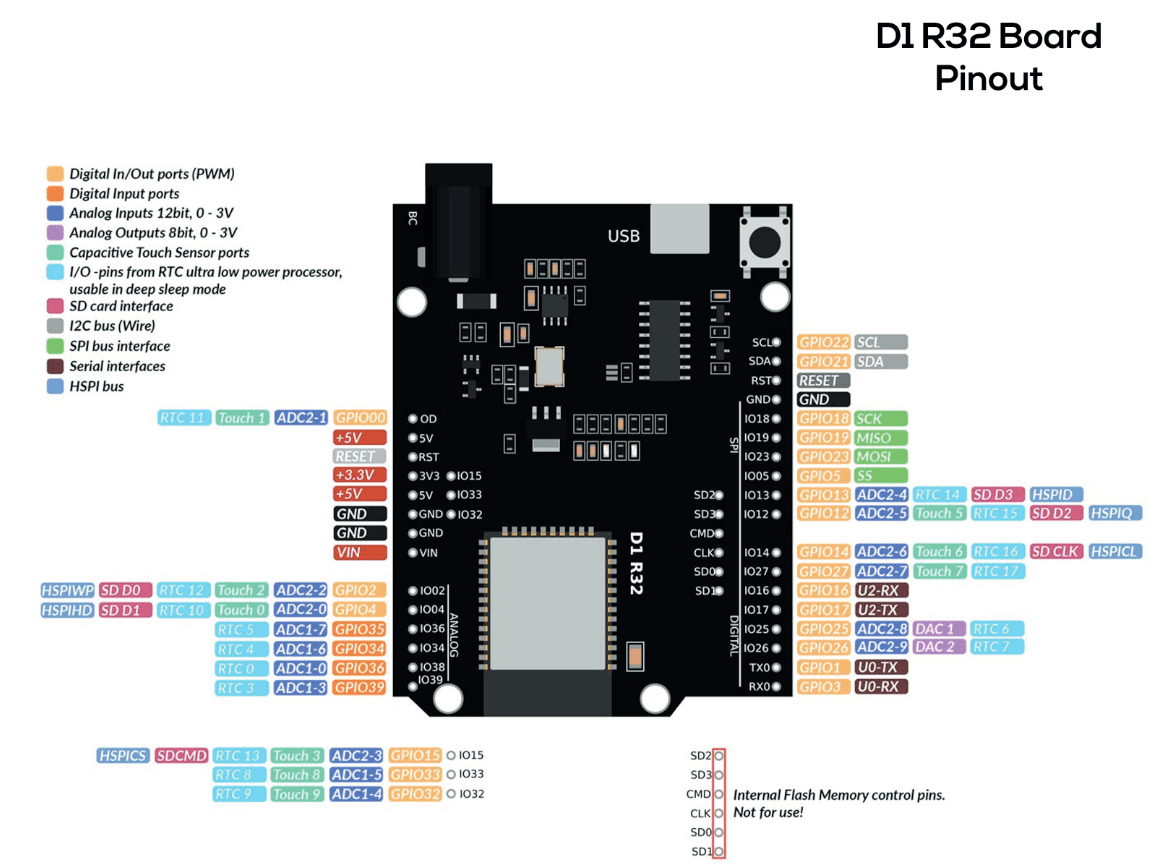
\includegraphics[width=\linewidth,height=5in]{img/esp.png}\\[1pt]
  \caption{ESP32}
  \label{fig:propojeniSFactory}
\end{figure*} 
\newpage

\section{Schéma zapojení}
Schéma našeho zapojení je na obrázku \ref{fig:schema}. Máme zde dvě komponenty a těmi jsou výše zmíněny TFT barevny display o rozlišení 128x128 pixelů a indikační led. Display má dva napájecí piny, těmi jsou pin led, který vuyžívá 3.3V a pin vcc, ten potřebuje 5V. Dále jak dioda, tak i display potřebuji připojenou zem (u displeje port gnd a led katoda). Pro propojení s SPI kanálem jsme využili zeleně zvýrazněné piny IO18, IO23 a IO5. Na pin IO18 se připojil hodinový signál sck. Pin I023 slouží pro sda probíhá tam komunikace MOSI (Master output slave input). MISO (Master input slave output), pak vůbec nepotřebujeme, protože komunikace je jednostraná od mikrokontroléru k displeji. A na port IO5 jsme zapojili pin cs, což nám reprezentuje SS (slave select). Dále zde jsou piny A0 a Res připojeny na IO25 a IO26. Pro diodu jsme vyhradili pin IO14.
\begin{figure*}[h]%\centering
  \centering
  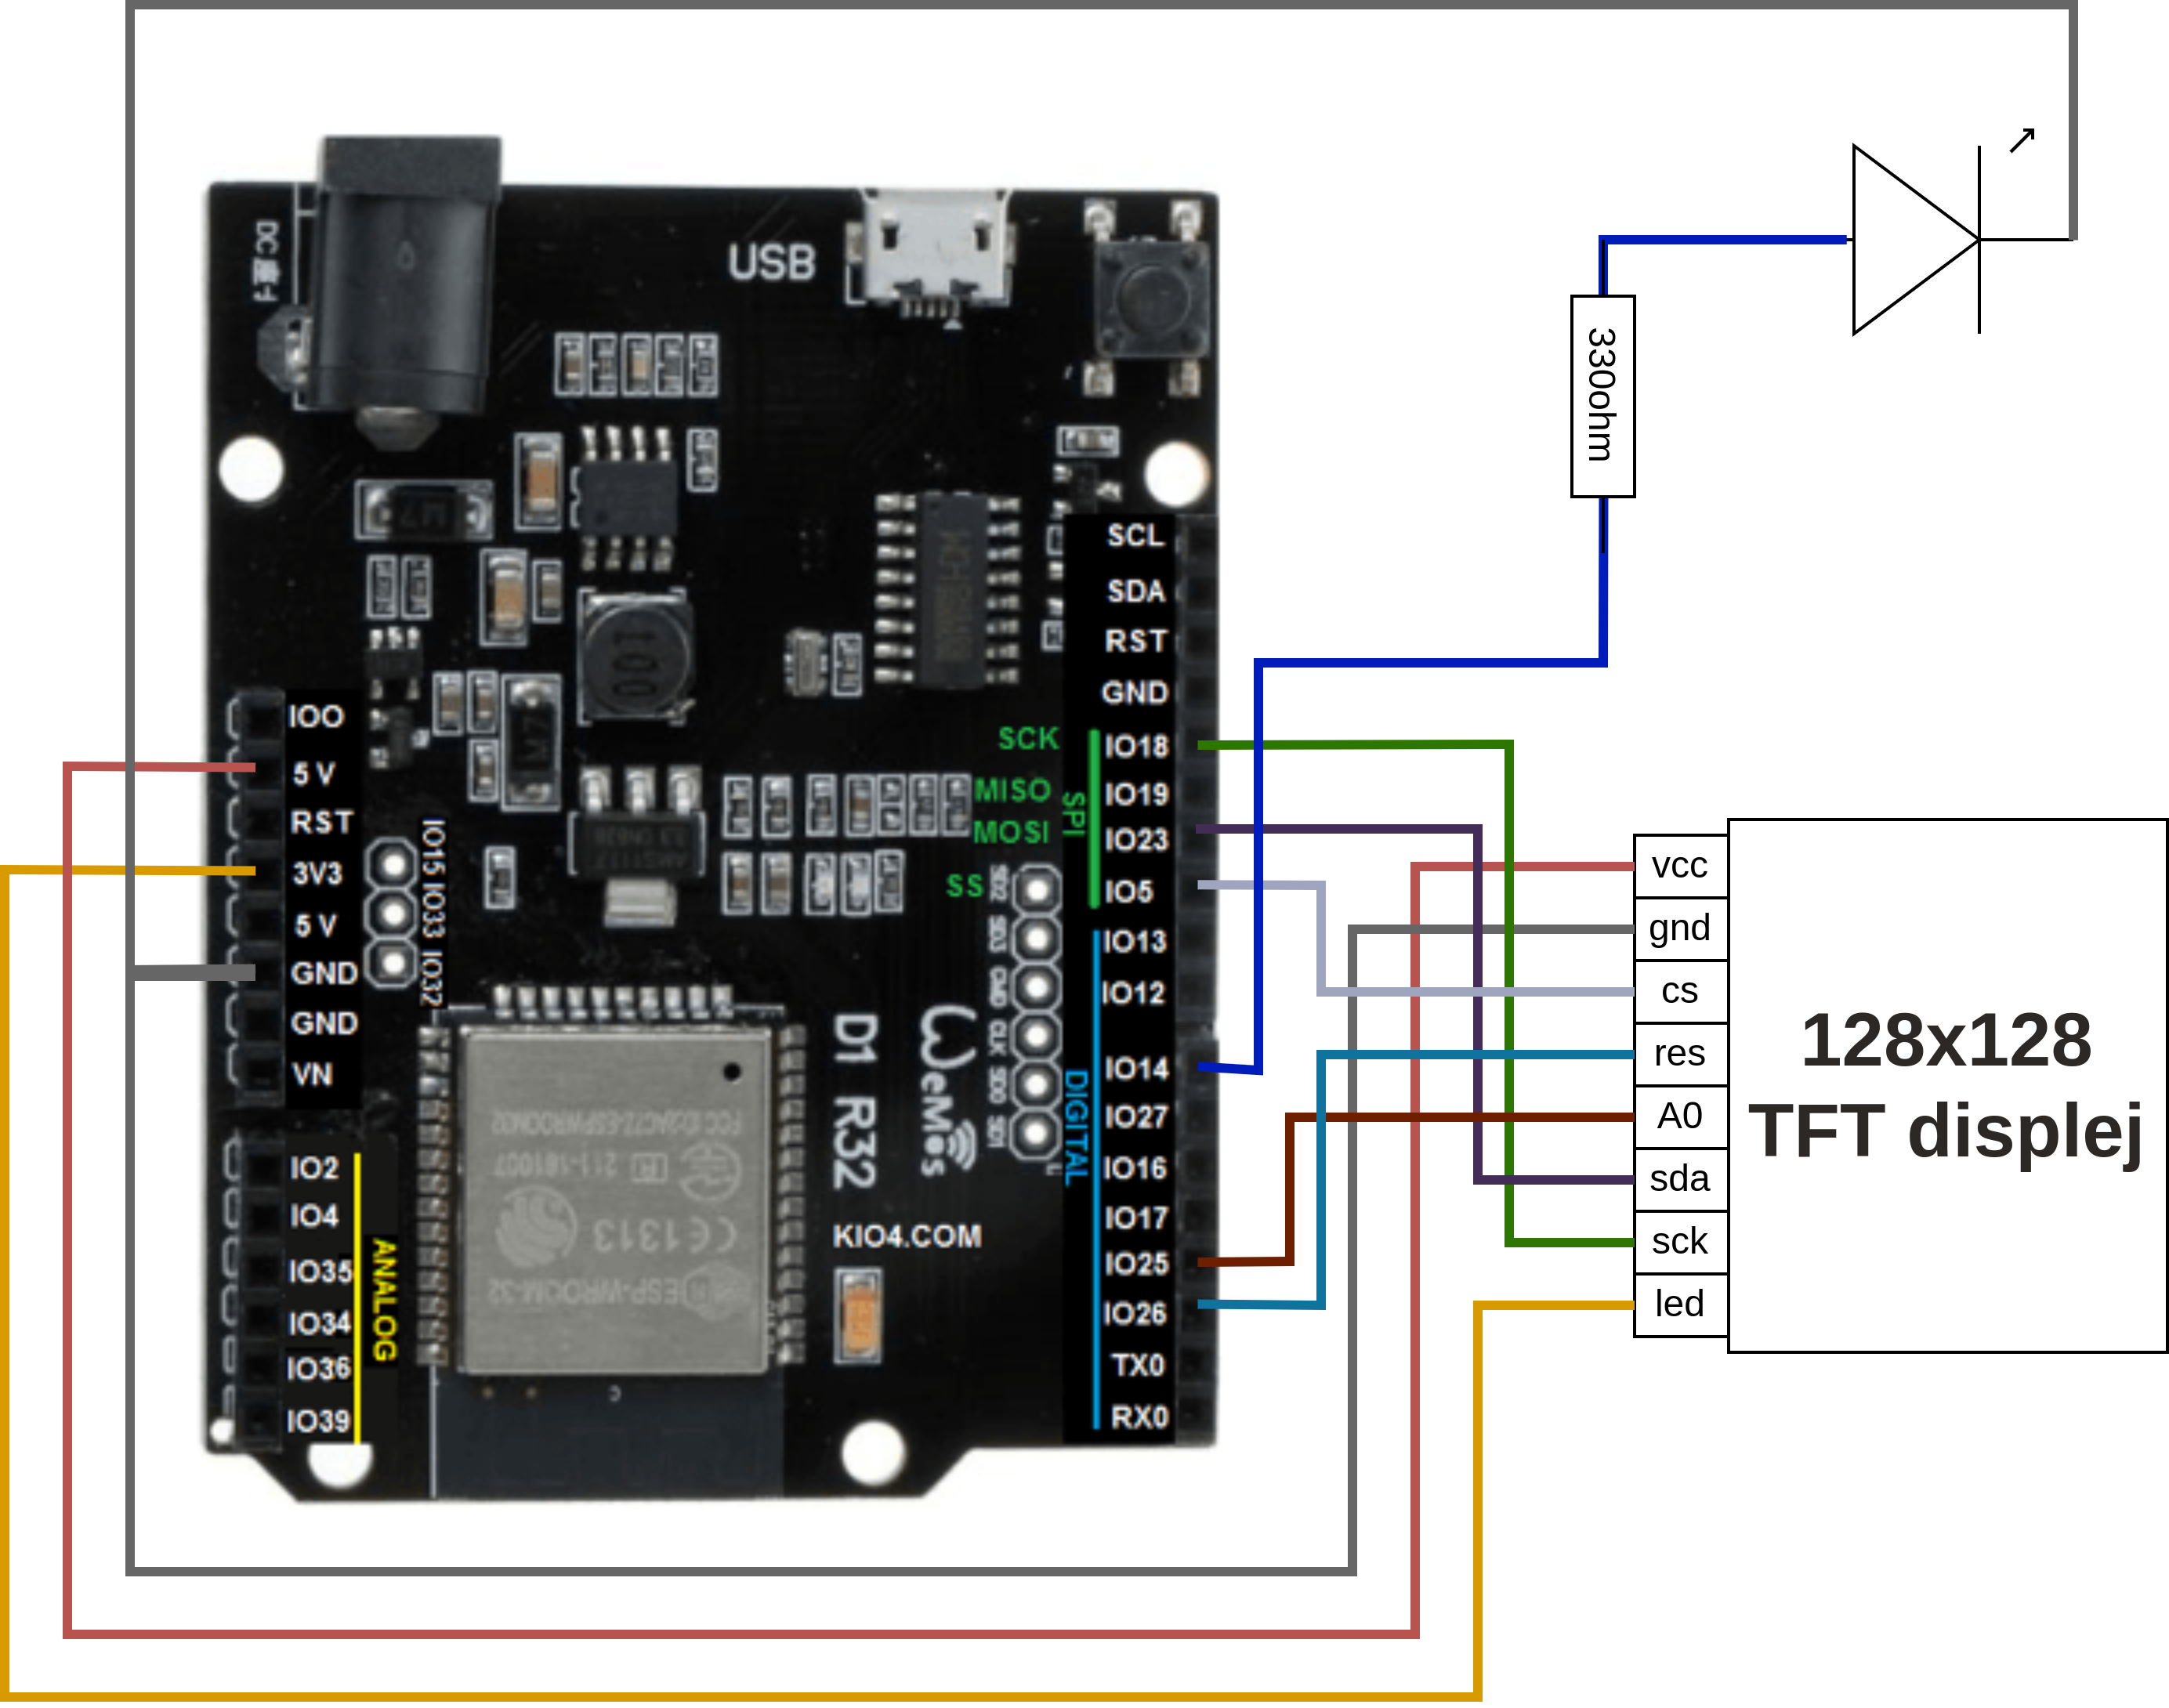
\includegraphics[width=\linewidth,height=5in]{img/scheme.png}\\[1pt]
  \caption{Schéma zapojení}
  \label{fig:schema}
\end{figure*} 

\section{Implementace}
Náš projekt jsme implementovali v prostředí Arduino IDE pomocí jazyka C a zároveň jsme využili knihovny, které Arduino poskytuje. těmi jsou: \\\\
\begin{listlisting}
\<Adafruit\_GFX.h\> - knihovna pro práci s grafikou displeje. \\
\<Adafruit\_ST7735.h\> - knihovna pro práci s naším konkretním displejem. \\ 
\<SPI.h\> - knihovna pro práci s SPI rozhraním. \\
\<WiFi.h\> - knihovna pro vytvření Wifi \\
\<WebServer.h\> - knihovna pro vytvoření webového serveru. \\
\end{listlisting}

Logika programu je velmi jednoduchá. Na začátku inicializujeme Wifi, webový server, displej (především inicializace SPI kanálu) a led. Po inicializaci dostane uživatel signál a to takový, že bude led na 2 sekundy svítit, což znamená úspěšnou inicializaci. Program pak vytvoří Wifi, tedy zařízení bude vystupovat v roli AP (access point) na síti 192.168.1.0/24, kde se může libovolné jiné zařízení připojit. Adresa 192.168.1.1 je rezervovaná pro mikrokontrolér všechny ostatní adresy se přidělují přes DHCP, které je vytvořeno pomoci knihovny \texttt{WiFi.h}. Na ip adrese mikrokontroléru je pak dostupná webová stránka, kterou program vytvořil pomocí funkce \texttt{generateHTML()} a požadavky na tento web se zpracovávají pomocí dalších funkcích programu a hlavně díky knihovny \texttt{WebServer}. Uživatel si za předpokladu, že je připojen k Wifi tohoto zařízení, může měnit stav displeje pomocí tlačítek. Obrazce na displej jsou vykreslovaný za pomocí knihovny \texttt{Adafruit\_GFX.h} a data jsou pak přeneseny pomocí SPI MOSI kanálu. Tuto logiku můžeme vidět na následujícím algoritmickém schéma.

\begin{figure*}[h]%\centering
  \centering
  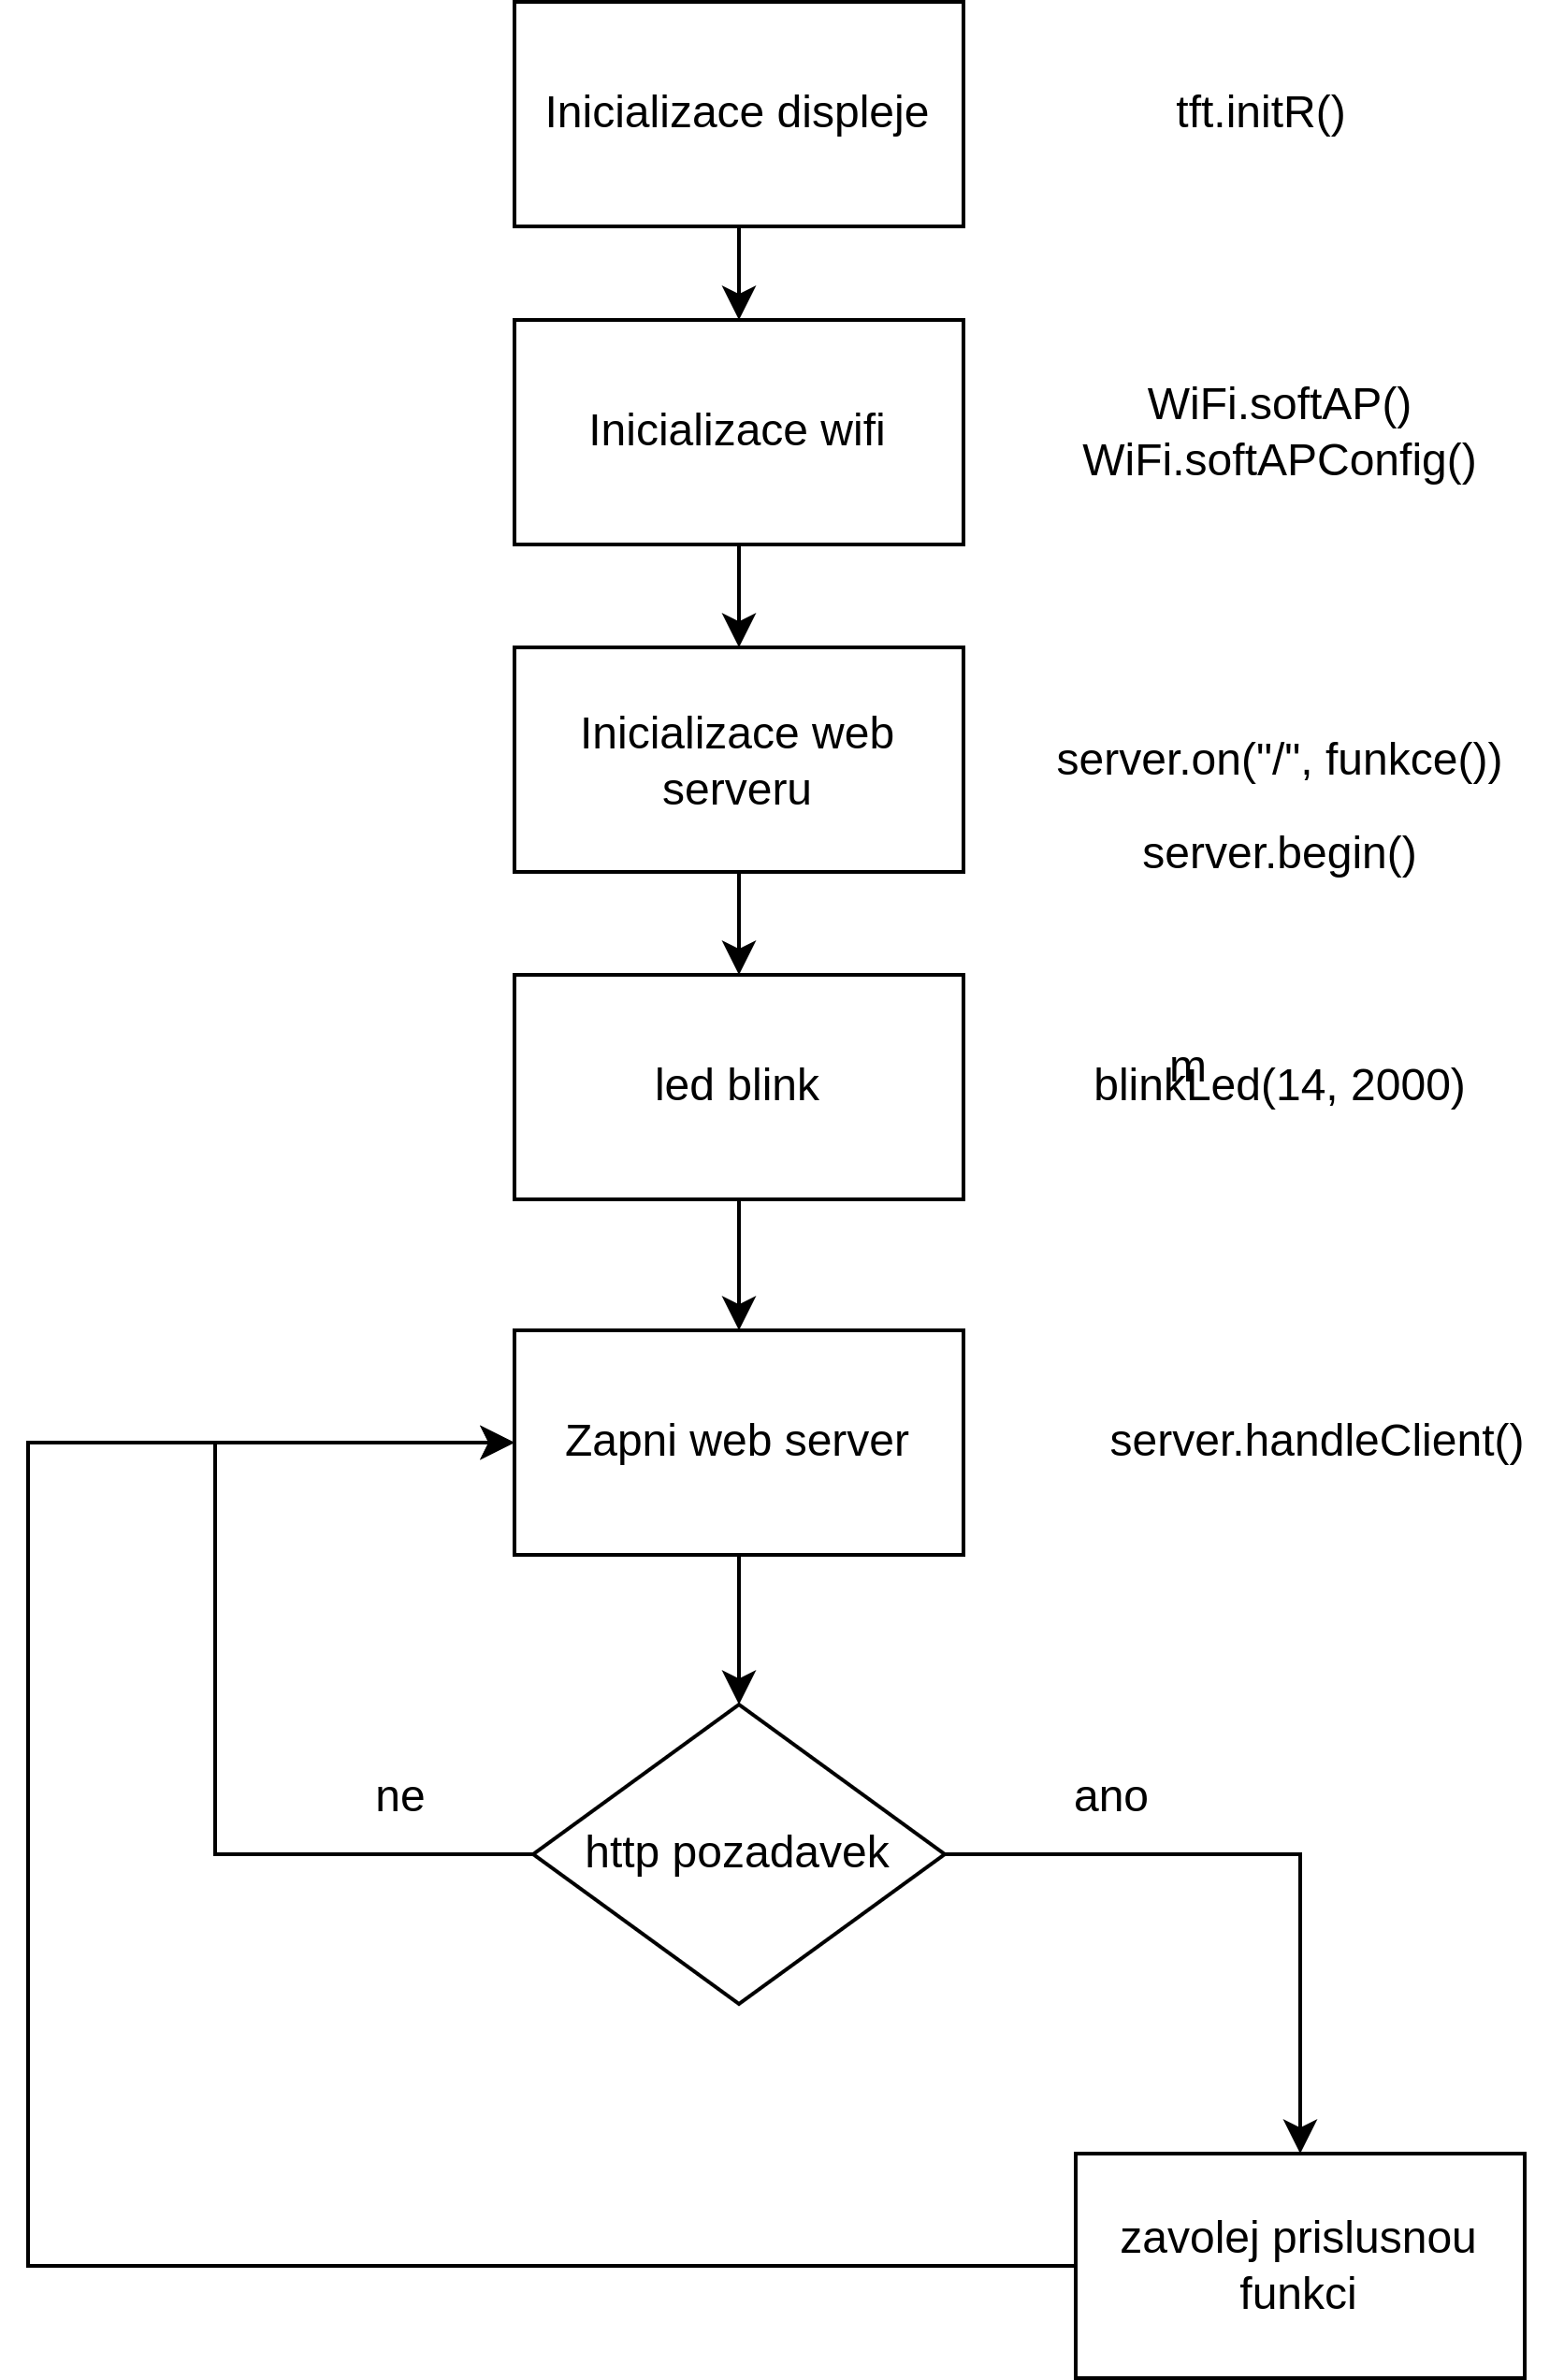
\includegraphics[width=4in,height=6in]{img/program.png}\\[1pt]
  \caption{Algoritmické schéma}
  \label{fig:schema}
\end{figure*} 

\section{SPI komunikace}
SPI je sériové periferní rozhraní, které umožňuje připojit více zařízení na jeden kanál. Vybrání zařízení se, kterým se bude komunikovat se dělá pomocí pinu SS (slave select). SPI je technologie na principu master slave. Master je v našem případě mikrokontrolér ESP32 a slave je TFT displej.

ESP se dá využít v obou rolích, jak slave tak master a jeho SPI schéma můžeme vidět na obrázku číslo \ref{fig:spiSchema}. SPI0 je zde používány jako buffer pro přístup k externí paměti (cache). SPI1 je používán jako Master, SPI2 a SPI3 pak můžou fungovat jako master nebo slave.  ESP může zpracovat více CS signálu, a tedy může mít připojených více slave najednou, například více displejů. SPI má signal BUS, který umí zpracovat signály D, Q, CS0-CS2, CLK, WP a HD. 

Naše ESP je nastaveno v režimu master. Pro posílání dat na displej používáme signál 0x6, který zapíše data do GP-SPI bufferu a pak je pomocí odešle na MOSI pin \cite{esp}.
\begin{figure*}[h]%\centering
  \centering
  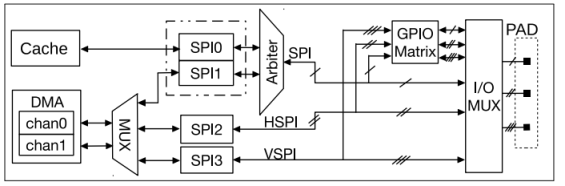
\includegraphics[width=5in,height=2in]{img/spi.png}\\[1pt]
  \label{fig:spiSchema}
\end{figure*} 


\section{WiFi}
Pro to aby WiFi fungovala musí hodinový signál APB\_CLK využívat signál PLL\_CLK jako svůj zdrojový hodinový signál. To se zajistí nastavením příznaku DPORT\_WIFI\_CLK\_EMAC\_EN v registru 5.19. Mac adresa wifi je pak uložená v registru WIFI\_MAC\_Address. Wifi zapneme pomoci nastavení příznaku RTC\_CNTL\_WIFI\_PD\_EN v registru 31.28 \cite{esp}.


